
\documentclass[12pt]{article}
\usepackage{graphicx}
\usepackage{amsmath}
\usepackage{mathtools}
\usepackage{gensymb}

\newcommand{\mydet}[1]{\ensuremath{\begin{vmatrix}#1\end{vmatrix}}}
\providecommand{\brak}[1]{\ensuremath{\left(#1\right)}}
\providecommand{\norm}[1]{\left\lVert#1\right\rVert}
\providecommand{\abs}[1]{\left\vert#1\right\vert}
\newcommand{\solution}{\noindent \textbf{Solution: }}
\newcommand{\myvec}[1]{\ensuremath{\begin{pmatrix}#1\end{pmatrix}}}
\let\vec\mathbf

\begin{document}
\begin{center}
\textbf\large{CONIC SECTIONS}

\end{center}
\section*{Excercise 10.2}
Q2.In fig \ref{fig:Fig1}, if TP and TQ are two tangents to a circle with centre O so that $\angle{POQ} = 110\degree$ then $\angle{PTQ}$ is equal to.
\begin{figure}[!h]
	\begin{center} 
	    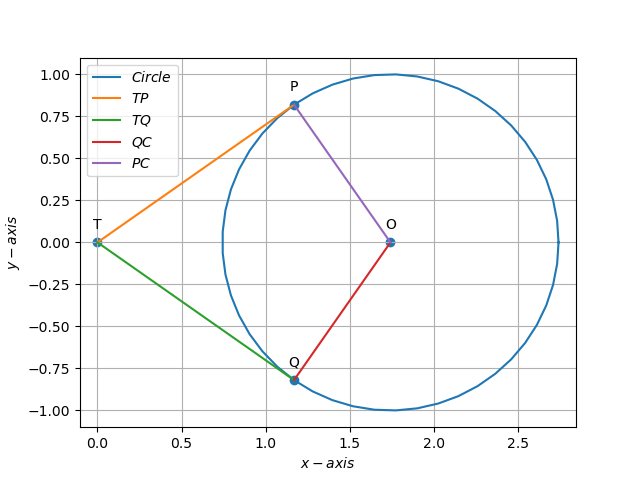
\includegraphics[width=\columnwidth]{figs/tan2}
	\end{center}
\caption{}
\label{fig:Fig1}
\end{figure}

\solution
Let
\begin{align}
	\text{radius} = r \text{ and } \vec{c} = \myvec{0\\0}
\end{align}
Now we know any point on circle is given as
\begin{align}
	\vec{X} = \vec{c}+r\myvec{\cos\theta \\ \sin\theta}
\end{align}
So,
\begin{align}
	\vec{P} &= \myvec{0\\0}+r\myvec{\cos0\degree\\\sin0\degree} = \myvec{r\\0}\\
	\vec{Q} &= \myvec{0\\0}+r\myvec{\cos110\degree\\\sin110\degree} = \myvec{r\cos110\degree\\r\sin110\degree}
\end{align}
For tangent TP
\begin{align}
	\vec{n}_1 &= \vec{P}-\vec{c} = \myvec{r\cos110\degree\\r\sin110\degree} = \myvec{1\\\tan110\degree}\\
	\vec{m}_1 &= \myvec{1\\-\cot110\degree}
\end{align}
For tangent TQ
\begin{align}
	\vec{n}_2 &= \vec{Q}-\vec{c} = \myvec{r\\0} = \myvec{1\\0}\\
	\vec{m}_2 &= \myvec{0\\1}
\end{align}
Now the angle between two lines with slope $\vec{m}_1 \text{ and } \vec{m}_2$ is given as
\begin{align}
	\label{eq:eq1}
	\cos\theta &= \frac{\vec{m}_1^\top \vec{m}_2}{\norm{\vec{m}_1}\norm{\vec{m}_2}}
\end{align}
Now,
\begin{align}
	\norm{\vec{m}_1} &= \sqrt{1^2 + \brak{-\cot110\degree}^2} = \csc110\degree\\
	\norm{\vec{m}_2} &= 1
\end{align}
Substituting the values in \eqref{eq:eq1}
\begin{align}
	\cos\theta &= \frac{\myvec{1&-\cot110\degree}\myvec{0\\1}}{\csc110\degree}\\
	&= -\cos110\degree\\
	&= \cos \brak{180-110}\\
	\implies \theta &= 70\degree
\end{align}
Hence, $\angle{PTQ} = 70\degree$ 
\end{document}






















